\section{Introduction}
\label{sec:introduction}

\begin{figure}[pos=t]
    \centering
    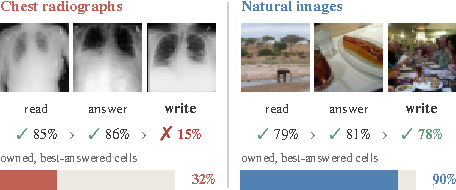
\includegraphics[width=\columnwidth]{figures/fig0_teaser.pdf}
    \caption{\textbf{Reading, answering, and ownership across image domains.} The top row shows the share of checkpoint--concept pairs that pass each RAW grade. The bars show ownership among the best-answered pairs.}
    \label{fig:teaser}
\end{figure}

Vision-language models (VLMs) can answer questions about a chest radiograph, but an accurate answer provides little information about how the model arrived at it. A linear probe, a simple classifier fitted to the model's internal image features, tests whether those features contain information about a finding.\cite{alain2017understanding,belinkov2022probing} In radiology, probes have located information about findings and detected acquisition and device cues that models could use as shortcuts.\cite{zhu2026lost,pedersen2026probes} Probes also yield a direction, a vector describing how the features would have to change to increase the probe's score for the finding.

\label{sec:related}
Activation steering changes a model's behavior by adding a vector to its internal features during prediction. Inference-time intervention and concept guidance use directions fitted by probes as steering vectors.\cite{li2023iti,vonrutte2024guide} Related steering methods use vectors derived from examples of a concept,\cite{zou2023representation,turner2023steering,panickssery2024caa} and concept activation vectors use a classifier direction to test how sensitive a prediction is to a concept.\cite{kim2018tcav} In VLMs, changing image features can alter the model's answers.\cite{rajaram2025lineofsight,ferrando2026explain} Ravichander et al.\cite{ravichander2021probing} showed that a probe can recover information the model itself does not use. Arad et al.\cite{arad2025saes} distinguished features that detect a concept from those that control an output. An audit of a clinical intervention also has to establish whether a change in the answer is specific to the labeled finding. Random vectors and a sham, a vector made by shuffling the coordinates of the fitted direction, lack a clinical label and cannot distinguish an effusion effect from one produced by another finding.

For Qwen2.5-VL-7B\cite{bai2025qwen25vl} on NIH ChestX-ray14,\cite{wang2017chestxray} adding the effusion direction increased the probability of a yes answer to the effusion question by \cfSeedWEff{}, above both random and sham controls (Fig.~\ref{fig:framework}). Adding the nodule direction on the same patients increased the effusion answer by \cfSeedWNodule{}. The effusion answer failed the ownership criterion because another finding's direction raised it more. Assessing the specificity of the effusion direction requires measuring its effects on the answers to other findings.

We developed Read--Answer--Write (RAW) to compare each finding's direction with competitors, directions fitted in the same way for other labeled concepts. RAW measures whether the model's features encode the finding, whether the model answers the question, and how its answers change when each direction is added. It applies to open-weight VLMs whose activations can be accessed. We evaluated \cfCheckpoints{} checkpoints, or saved sets of model weights, from \cfFamiliesWord{} model families on NIH ChestX-ray14 and CheXpert Plus,\cite{chambon2024chexpertplus} using COCO photographs\cite{lin2014coco} as a natural-image control.

Chest findings were readable and answerable at least as often as COCO objects, with ownership in \cfChestOwnedPct{}\% of chest pairs versus \cfCocoOwnedPct{}\% of COCO pairs (Fig.~\ref{fig:teaser}). Random and sham references alone would have certified \jnRefChest{} chest directions, half of which failed the labeled comparisons. The ownership gap persisted at comparable answer difficulty, and non-clinical attributes of the same radiographs showed similarly low ownership. Changing the components downstream of the vision tower changed ownership even when the models received the same visual features and steering directions.
